\section{Kapitel 7}
\subsection{Aufgabenstellung}
Wie sollen 7 Klassen Definieren, dabei sollen wir uns überlegen welche davon Instanziierbar sind und welche
nicht. Anschließen soll jede Klasse sinnvolle Methoden und Attribute enthalten.

\subsection{Anforderungsdefinition}
\begin{enumerate}
	\item Definiere folgende Klassen: Viereck, konvexes Viereck, Trapez, Parallelogramm, Rhombus, Rechteck, Quadrat
	\item Definiere sinnvolle Methoden und Attribute
\end{enumerate}

\subsection{Entwurf}
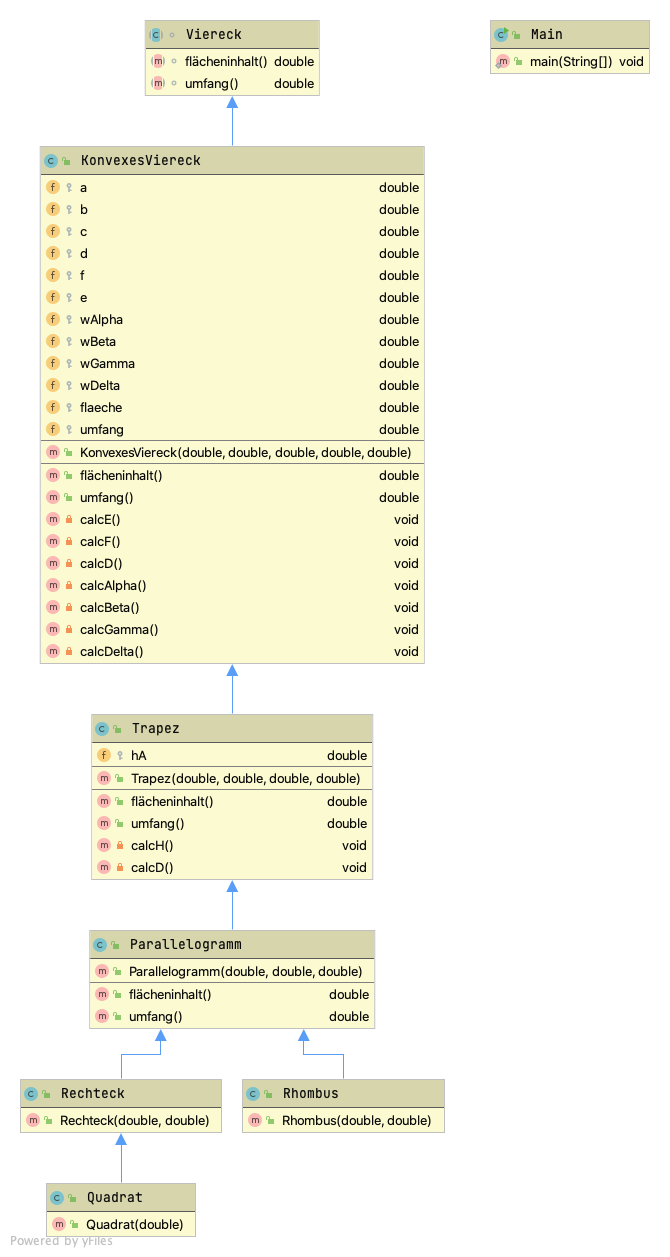
\includegraphics[scale=0.55]{uml/uml_c7_p1.png}

\subsection{Quelltext}
\subsubsection{Main.java}\
\lstinputlisting[language = Java , frame = trBL , escapeinside={(*@}{@*)}]{../chapter_07/src/chapter_07/Main.java}
\subsubsection{Viereck.java}\
\lstinputlisting[language = Java , frame = trBL , escapeinside={(*@}{@*)}]{../chapter_07/src/chapter_07/figures/Viereck.java}
\subsubsection{KonvexesViereck.java}\
\lstinputlisting[language = Java , frame = trBL , escapeinside={(*@}{@*)}]{../chapter_07/src/chapter_07/figures/KonvexesViereck.java}
\subsubsection{Trapez.java}\
\lstinputlisting[language = Java , frame = trBL , escapeinside={(*@}{@*)}]{../chapter_07/src/chapter_07/figures/Trapez.java}
\subsubsection{Parallelogramm.java}\
\lstinputlisting[language = Java , frame = trBL , escapeinside={(*@}{@*)}]{../chapter_07/src/chapter_07/figures/Parallelogramm.java}
\subsubsection{Rhombus.java}\
\lstinputlisting[language = Java , frame = trBL , escapeinside={(*@}{@*)}]{../chapter_07/src/chapter_07/figures/Rhombus.java}
\subsubsection{Rechteck.java}\
\lstinputlisting[language = Java , frame = trBL , escapeinside={(*@}{@*)}]{../chapter_07/src/chapter_07/figures/Rechteck.java}
\subsubsection{Quadrat.java}\
\lstinputlisting[language = Java , frame = trBL , escapeinside={(*@}{@*)}]{../chapter_07/src/chapter_07/figures/Quadrat.java}

\subsection{Testdokumentation}
?

\subsection{Benutzungshinweise}
?

\subsection{Anwendungsbeispiel}
Nach dem man das Programm gestartet hat, sollte folgende Ausgabe erscheinen:
\begin{lstlisting}[frame = trBL , escapeinside={(*@}{@*)}]
	[sebastian@laptop bin]$ java Main
	20.0 50.0
	20.0 50.0
	20.0 15.0
	30.0 50.0
	20.0 25.0
	[sebastian@laptop bin]$ 
\end{lstlisting}